\chapter{Методика исследования}

%В процессе исследовани нами были испытаны грунты методами 
Для определения характеристик переуплотнения грунта, были проведены испытания методом компрессионного сжатия. 

Компрессия – способность грунта сжиматься под постоянной, но ступенчато возрастающей нагрузкой без возможности его бокового расширения в условиях открытой системы.

Компрессионное сжатие производилось по ГОСТ 12248-2010 и ГОСТ 15236-2018, в приборах ГТ1.1.4-01 ООО «НПП ГеоТек» (Пенза) при максимальных ступенях нагрузок до 2.5 МПа на образцах с заданной влажностью. 

Полученные данные были обработаны методами Казагранде и Беккера. 

\section{Метод Казагранде}

По методу Казагранде строится полулагорифметический график зависимости коэффициента пористости от вертикального напряжения.  
Метод, предложенный Артуром Казагранде хорошо зарекомендовал себя для глинистых грунтов, однако, графические методы несколько неудобны для инженерного использования.

В логарифмических координатах идеализированная компрессионная кривая в довольно широком интервале вертикальных напряжений представлет собой линейную зависимость в случае непереуплотненного грунта, и билинейную "--- в случае переуплотненного:
первый участок соответствует ветви рекомпрессии, а второй "--- ветви первичного сжатия.

Интуитивно, самым простым способом определения давления предуплотнения, является поиск точки пересечения двух касательных к начальному и конечному участку компрессионной кривой. 
Однако, сложности с выбором касательной к начальному участку кривой, побудили А. Казагранде в 1936 г. создать усовершенствованный метод. 
По-видимому, ученый полагал, что угол наклона касательной заключен в двух крайних положениеях. 
Минимальный угол наклона соответствует горизонтальной прямой, а максимальный "--- углу наклона касательной в точке с наименьшим радиусом кривизны. 
Далее он брал среднее значение этих крайних случаев "--- проводил биссектриса между ними. 
Пересечение биссектрисы с касательной конечного участка дает искомую величину напряжения предуплотнения.


В этом методе присутствуют сложности, связанные с графическими построениями и наличием субъективного фактора.
Испытания должны быть проведены до таких величин вертикальных напряжений, при которых обеспечивается достоверный выход на линию первичного сжатия. Только касательная к такому участку даст единственно верный наклон для построения касательной к конечному участку. Угол наклона касательной соответствует первой производной в конечной точке.

Точка максимальной кривизны, как правило, выражена не ясно и выбирается геологом субъективно. По смыслу точка максимальной кривизны соответствует точке минимума второй производной аналитического представления компрессионной кривой.

Следующим субъективным фактором является проведение касательной к точке максимальной кривизны, вследствие тех же причин. Это аналитически и по смыслу соответствует значению первой производной компрессионной кривой, точки минимума второй производной.

Как говорилось ранее, биссектриса является средним значением крайних случаев, а именно минимальным и максимальным углом наклона горизонтальной прямой и касательной в точке с наименьшим радиусом кривизны. 
И таким образом, является оценкой,  осредняющей два крайних значения. 
Помимо этого, построение биссектрисы в пространстве различных размерностей является абсурдным, что приводит к искажениям вследствие выбора масштабов по осям напряжений и коэффициента пористости. \cite{boone_critical_2010}
Зависимость от выбранного масштаба  иллюстрируется на рисунке \ref{fig:ellipse}.

 \begin{figure}
    \label{fig:ellipse}
    \center
    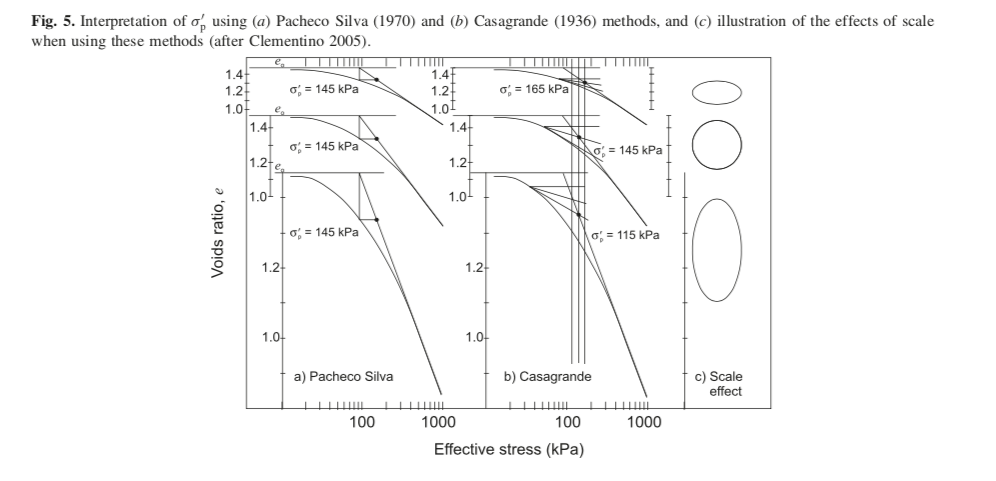
\includegraphics[scale=0.5]{3.png}
    \caption{Сравнение методов Казагранде и Пашеко Силва.}
\end{figure}
    
\section{Метод Беккера}

Метод Беккера относится в группе энергитических методов.

Согласно методу Беккера, значение напряжение предуплотнения $\sigma_p$ находится по графику зависимости увеличения работы на единицу объема (произведения давления на деформацию) от приращения вертикального давления.

В своей работе Беккер указывает, что величина давления, равного суммарной работе, определяется давлением в конце приращения деформации. 
Полученная зависимость, как правило, имеет два прямолинейных участка. 
Напряжение, соответствующее точке пересечения двух прямых, проведенных к линейным участкам кривой, соответствует давлению предварительного уплотнения. (<<work as a criterion for determining in situ and yield stresses in clays D.Becker at all, 1987>>).

Вследствие эквивалентности пространства построения $W - \sigma$ эквивалентно пространству $e - \ln \sigma$, что подтверждается следующим уравнением \cite{article_Wang_2004}: 

$$de = C_c d \log\sigma$$
$$dE = \int_{\sigma_1}^{\sigma_2} \frac{\sigma}{1+e_0} de 
= \int_{\sigma_1}^{\sigma_2} \frac{\sigma}{1+e_0} \frac{C_c d\sigma}{\sigma}
= \frac{C_c (\sigma_2 "--- \sigma_1)}{1+e_0}$$


Соответственно, к недостаткам метода, так же как и для метода Казагранде, можно отнести наличие субъективного фактора при графических построениях, в частности сложность в выборе линейных участков, к которым проводятся прямые. 

В зависимости от типов грунтов, тот или иной метод может оказаться чувствительнее, поэтому в ГОСТ 58326-2018 рекомендуется проводить обработку результатов всегда двумя способами и выбирать из них меньшее значение переуплотнения, то есть то, которое обеспечивает наибольший запас при проектировании.

\section{Подготовка и проведение испытаний}

Для проведения испытаний были подготовлены образцы нарушенного сложения из грунтов, отобранных на месте изысканий. Грунтовая паста доводилась до текучего состояния с влажностью превышающей в 1,5--2 раза влажность на пределе текучести. 
Паста текучей конситенции использовалась с целью представления образца нормально уплотненного грунта.

Испытания проводились в два этапа.
Схема испытаний для первого этапа была составлена таким образом, чтобы смоделировать процесс седиментации образца, достижения им заданного максимального исторического давления, процесса извлечения образца на поверхность.

Второй этап моделировал собственно компрессионное сжатие образца в одометре, после его извлечения из массива грунта.

Для этого грунтовая паста нагружалась ступенями начиная 6 кПа.
Каждая последующая ступень принималась в два раза больше предыдущей.
Максимальное напряжение по первой ветви нагрузки соответсвовало 600 кПа.
Первая ветвь нагружения соответствует ветви первичного компрессии.

Затем производилась постепенная полная разгрузка образца.

После этого образец нагружался по схеме первой ветви, но до максимального давления 2500 кПа.
Цель работы была найти перегиб на второй ветви, соответствуюшей переходу образца из зоны рекомпрессии в зону первичного сжатия.
Такой последованностью действий возможно показать всю историю нагрузок и подробно воссоздать природные наряжения, при которых существовал грунт. 

Как говорилось ранее, в данной работе рассматривается единственный фактор: максимальное историческое напряжение. Поэтому для того, чтобы оценить точность методов Казагранде и Беккера, грунты нарушенной структуры были испытаны по данной схеме, что не противоречит ГОСТ 58326-2018.
 
